%%%  edit this file and my_styles.tex  only  !!!


%%% coment or uncomment appropriate choice  1=yes, 0=no
% \setcounter{Anglicky}{0}  %  NO
\setcounter{Anglicky}{1}   % YES

%
%  do tohoto souboru nepatri konstrukce 
%
%\newtheorem{cosi}{}
%\newenviroment{cosi}
%\def\cosi#1{}
%\def\cosi{}
%\gdef\cosi
%
% vyse uvedene patri do my_styles.tex, a navic je potreba pred cosi pridat Vase jmeno ci
% neco Vaseho jedinecneho -> zamezi se tak kolizim mezi stejne pouzitymi stringy "cosi" od
% ruznych prispevku, stejne tak ruznym nezadoucim predefinovanim !!!
%
 
%
% pri importu grafickych souboru .eps. .ps. vynechat extenzi. Ono si ji to doplnuje podle
% druhu kompilatoru  LaTeX nebo pdfLaTeX. V pripade kompilace s pdfLaTeX musi byt k
% dispozici odpovidajici .pdf nebo .jpg soubor.
%
%

\Nazev{Fuzzy Classification of Web Reports with Linguistic Text Mining}    % required
\RunningTitle{Fuzzy Classification of Web Reports}      % short name for page heading, or 
                                        % the same as Nazev, required

\Doktorand{Jan D\v{e}dek}               % full name, no abreviations,  required
\DoktorandPredniTitul{Mgr.}             % required
\DoktorandZadniTitul{}                  % required, if any

\DokAdresa{\MFFUKMalaStrana}  % required,  \UIAVCR, \KMFJFI,
                                                   % MUUKKarlin, \MFFUKMalaStrana  
                                                   % and  \EUROMISE  are available, 
                                                   % use it regardless of selected language

\DokEmail{jan.dedek@mff.cuni.cz}        % required

\OborStudia{Software engineering}           % required

\Skolitel{Peter Vojt\'{a}\v{s}}                      % required
\SkolitelPredniTitul{Prof. RNDr.}       % required !!!!!!
\SkolitelZadniTitul{DrSc.}              % required !!!!!!

\SkoAdresa{\MFFUKMalaStrana} % required,  \UIAVCR, \KMFJFI,
                                        % MUUKKarlin, \MFFUKMalaStrana  
                                        % and  \EUROMISE  are available, 
                                        % use it regardless of selected language

\SkoEmail{peter.vojtas@mff.cuni.cz}      % required

\ThanksGiving{This work was partially supported by Czech projects: IS-1ET100300517, GACR-201/09/H057 and GAUK 31009.}
% and MSM-0021620838.} 
                                        % or empty if no support available

\MakeContributionTitle

\begin{multicols}{2}

\begin{abstract}
In this paper we present a fuzzy system which provides a fuzzy classification of textual web reports. Our approach is based on usage of third party linguistic analyzers, our previous work on web information extraction and fuzzy inductive logic programming. Main contributions are formal models and prototype implementation of the system and evaluation experiments. 

%\smallskip
\medskip
%\bigskip

The abstract was originally published in the paper \cite{Dedek:FuzzWI}. Due to the copyright issues, only the abstract is presented here, extended with some additional information that is not included in the original paper.
\end{abstract}


\section{Introduction}
In this contribution we would like to present our latest work \cite{Dedek:FuzzWI} and extend it with some additional information about the issues that are closely related to the original paper. As the original paper has only four pages, here we present more details about the issues that are closely related to the paper.

The original paper deals with a structured data that could be extracted from web reports. The original paper is closely concentrated on the use of the structured data for a fuzzy classification of the reports. The original paper refers to our previous works where our method for extraction of a structured data form web reports is presented and gives very little details about it. In this contribution we present:
\begin{itemize}
	\item more details about our extraction method (see in the section~\ref{dedek:IEMethod}),
	\item a richer discussion of the related work (in the section~\ref{dedek:related}) and
	\item the current state of our development and our plans for the future work (in the last section).
\end{itemize}

\subsection{Motivation}
Big amount of information on the web increases the need of automated precessing. Especially textual information are hard for machine processing and understanding. Crisp methods have their limitations. In this paper we present a fuzzy system which provides a fuzzy classification of textual web reports. 

Messages of accident reports on the web (Fig~\ref{dedek:message}) are our motivating examples. We would like to have a tool which is able to classify such message with degree of being it a serious accident. 

Our solution is based first on information extraction (see emphasized information to be extracted in the Fig~\ref{dedek:message}) and second on processing this information to get fuzzy classification rules. Details about the fuzzy classification are presented in \cite{Dedek:FuzzWI}, here we will present only some additional information.

\begin{figure}
\medskip
\centerline{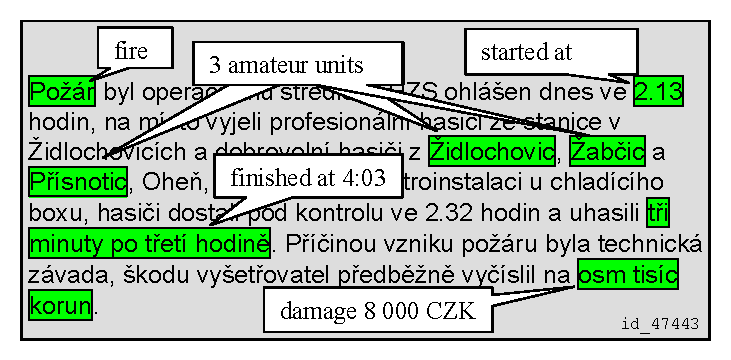
\includegraphics[width=\hsize]{img/message}}
\caption{Example of analyzed web report.}
\label{dedek:message}
\end{figure}


\section{Our Information Extraction Method} \label{dedek:IEMethod}
\subsection{Linguistic Analysis}
In this section we will briefly describe the linguistic tools that
we have used to produce linguistic annotations of texts. 
These tools are being developed in the Institute of Formal
and Applied Linguistics in Prague, Czech Republic. They
are publicly available -- they have been published on a CDROM
under the title PDT 2.0 \cite{dedek:PDT20_CD} (first five tools) and in
\cite{dedek:KlTransformationBasedTectogrammatical2006} (Tectogrammatical analysis). These tools are used as a
processing chain and at the end of the chain they produce
tectogrammatical \cite{dedek:MiBeAnnotationtectogrammatical2006} dependency trees. 


\begin{description}
 
	\item[Tool 1.] Segmentation and tokenization consists of tokenization
(dividing the input text into words and punctuation)
and segmentation (dividing a sequences of tokens
into sentences).

	\item[Tool 2.] Morphological analysis assigns all possible lemmas
and morphological tags to particular word forms (word
occurrences) in the text.

	\item[Tool 3.] Morphological tagging consists in selecting a single
pair lemma-tag from all possible alternatives assigned
by the morphological analyzer.

	\item[Tool 4.] Collins' parser -- Czech adaptation. 
Unlike the usual approaches to the description of
English syntax, the Czech syntactic descriptions are
dependency-based, which means, that every edge of
a syntactic tree captures the relation of dependency
between a governor and its dependent node. Collins'
parser gives the most probable parse of a given input
sentence.

	\item[Tool 5.] Analytical function assignment assigns a description
(analytical function -- in linguistic sense) to every edge
in the syntactic (dependency) tree.

	\item[Tool 6.] Tectogrammatical analysis produces linguistic annotation
at the tectogrammatical level, sometimes called
``layer of deep syntax''. Such a tree can be seen on
the Fig~\ref{dedek:tree}. Annotation of a sentence at this layer
is closer to meaning of the sentence than its syntactic
annotation and thus information captured at the tectogrammatical
layer is crucial for machine understanding
of a natural language \cite{dedek:KlTransformationBasedTectogrammatical2006}.
\end{description}

\subsection{Web Information Extraction}

Having web resource content analyzed by above linguistic tools, we have data stored in the form of tectogramatical trees. To achieve our objectives we have to extract information from this representation. 
Here we refer to our previous work \cite{dedek:DeVoLinguisticextraction2008,dedek:DeVoComputingaggregations2008,dedek:DeEcExperimentswith2008}. A long path of tools starting with web crawling and resulting with the extracted structured information is developed in our previous work. 
In Fig~\ref{dedek:tree} we can see nodes of tree where a piece of information about damage (8000 CZK) is located. We have used Inductive logic Programming to learn rules which are able to detect such nodes. 
%In this paper we will concentrate on the usage of such extracted information to be able to classify content. 
The extraction process requires a human assistance when annotating a training data.

Note that our method is general and is not limited to Czech and can be used with any structured linguistic representation. 


\begin{figure}
\medskip
\centerline{\framebox{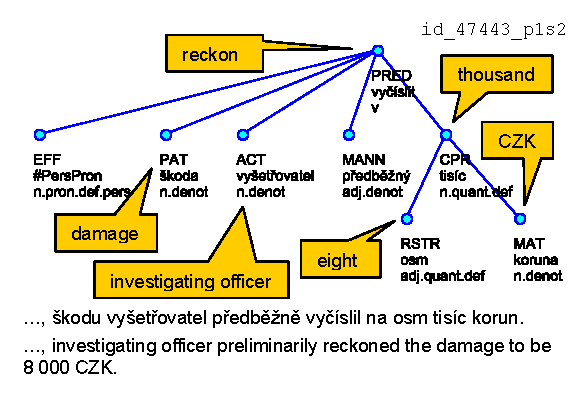
\includegraphics[width=\hsize]{img/tree}}}
\caption{Example of a linguistic tree of one of analyzed sentences.}
\label{dedek:tree}
\end{figure}



\section{Related Work} \label{dedek:related}

There is a plenty of systems dealing with text mining and text classification, let us mention at least some. In \cite{dedek:ReYaLiOntoText08} authors use ontology modeling to enhance text identification. In \cite{dedek:CAP} authors use preprocessed data from National Automotive Sampling System and test various soft computing methods to modeling severity of injuries (some hybrid methods showed best performance). Methods of Information Retrieval (IR) are very numerous, with extraction mainly based on key word search and similarities. Connecting IR and text mining techniques with web information retrieval can be found in Chapter Opinion mining in the book of Bing Liu \cite{dedek:WebDataMining}. 


\section{Conclusion and Future Work}

Currently we are working on the integration of our method with further linguistic tools and we work on a graphical user interface so the whole system could be distributed as a software package and used by arbitrary users.

We have made first experiments with the TectoMT system \cite{dedek:ZaPtTectoMTHighly2008}, which can replace the older tools from the PDT2.0 CD-ROM mentioned above and currently used in our system. TectoMT can bring us many befits like named entity recognition, better morphology and parsing (made by the McDonalds' parser \cite{dedek:mcdonald}), but the biggest advantage is that we can use the same linguistic formalism (tectogrammatical trees) for English (and probably for other languages in the future).

On the other hand our approach is not limited to the tectogrammatical trees and we have made first experiments with \emph{Stanford typed dependencies} \cite{dedek:staford_dependecies} as an alternative linguistic formalism.

We will probably use The GATE architecture \cite{dedek:GATE} as the platform for integration of our method with other systems and we can use it also as the graphical user interface. The GATE features will also bring a very modular fashion to the final system.

%The Stanford Parser: A statistical parser \cite{dedek:staford_parser}


\bibliographystyle{ieeetr}
\bibliography{Dedek_DD_UIAVCR}




\end{multicols}

% Local Variables:
% TeX-master: "sbornik-dd-2007"
% TeX-PDF-mode: t 
% End:






